\section{Delay and Missed Packets}
The delay in the system constitutes one of the main network issue in the system. It forces the controller design to be more robust and, in most cases, to make it slower. In order to consider the delay in the controller design, the TrueTime simulation toolbox for MATLAB is utilized. This toolbox allows to simulate the control design, the derived model and the wireless network together in order to find a control design that is still stable.

In the simulation, a model for the delay needs to be found in order to implement it in TrueTime. The chosen approach is to model the delay as the maximum possible delay appearing in the system, so the worst case scenario is considered. Its value is obtained by adding the time required to make the information, from the sensor, available in the serial port of the microcontroller and the maximum time elapsed since the data is available until it is used by the control loop. \autoref{fig:delaycontrol} shows the different networked induced delays in the system and the maximum delay.  

The time required to make the data available can be divided into two, as seen in the upper part of \autoref{fig:delaycontrol}. The time required to run the code in the computer, which retrieves the sensor data and constructs the packet, and the transmission delay. The precise value of the first can be found as it is the code execution time on the computer. The value obtained is \SI{15}{ms}. The transmission time can be found using the transmission speed of the Xbee modules. According to the datasheet \cite{XBee}, it is \SI{115.2}{kbit/s}. With this speed and transmitting 21 bytes, the transmission delay is \SI{1.46}{ms}. The first part of the delay in then \SI{16.46}{ms}, see \autoref{fig:delaycontrol}.

Once the information is on the microcontroller, the maximum time elapsed until the controller uses the data is the sampling period minus the execution time of the control loop. The reason for this is because in the worst possible case, the packet arrives just after a control loop finishes, then it is necessary to wait until the next control loop is executed. The final value of the second part of the delay is then ??, see \autoref{fig:delaycontrol}.
 
\begin{figure}[H]
	\centering
	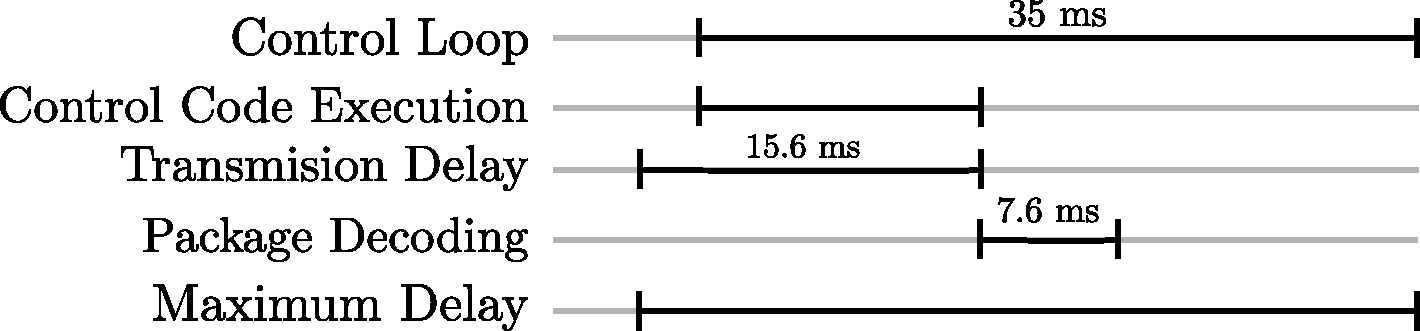
\includegraphics[width=.6\textwidth]{figures/maxDelay.pdf}
	\caption{Delays in the packages transmitted to the microcontroller and maximum delay.\fxnote{Check times when we have them all}}
	\label{fig:delaycontrol}
\end{figure}

After all considerations, the value of the maximum delay which is used in the simulation is \SI{50}{ms}??\fxnote{Check delay when we have them all}.

When considering issues in the network, it is necessary to look into the missed packets. A missed packet can occur if either a new packet is not received between two control loops, making second control loop use old data, or a received packet is corrupted.

This issue can be included in the simulation by utilizing TrueTime. Here the missed packets can be simulated as a constant probability of missing packets. To get this probability, tests are conducted in which 1000 packets are transmitted. The amount of packets received correctly and processed in the microcontroller together with the number of control loops executed, provides an estimate of the probability of missing packets. The data obtained with the tests is shown in more detail in \fxnote{accepttest?? WITH THE TEST}. The probability of missing a packet is found to be ??.

The protocol has been design and the main network issues, the delay and missed packets, have been analysed. Now it is possible to use this information when designing a stable controller.

% This implies that the most recent data is available for the control in every loop.

%The packets which are missed in the system causes the controller to use old data in the loop. This effect is also included in the simulation by utilizing TrueTime. In the system, packet loss is caused by the scheduling of the tasks in the microcontroller since information can not be processed when the controllers are running. Package loss across the wireless channel does not occur due to the low transmission frequency used.
 
%since the information is obtained until it is sent through the network, the transmission delay and the time needed to process the information in the microcontroller. being exponentially distributed. \autoref{eq:exponentialdist} shows the probability and cumulative density functions of the exponential distribution.
%\begin{flalign}
%		f=-\lambda\mathrm{e}^{-\lambda t}\mathrm{;}\ \ \ \ \  F=1-\mathrm{e}^{-\lambda t}
%		\label{eq:exponentialdist}
%\end{flalign}
%\begin{where}
%	\va{f} {is the probability density function} { }
%	\va{F} {is the cumulative density function} { }
%	\va{\lambda} {is the rate parameter} { }
%	\va{t} {is time} { }
%\end{where}
%The parameter lambda can be interpreted as the inverse of the mean time between observations, that is, the mean delay in the system. The value for this parameter has been found experimentally by measuring and averaging the experienced delays in \fxnote{PUT NUMBER} transmissions. The detailed experiments can be seen in \fxnote{APPENDIX WITH DATA}. The average delay obtained is \fxnote{PUT NUMBER} which leads to a value for $\lambda$ of \fxnote{PUT NUMBER}
 
%To generate the exponential distributed delays, the inverse transformation theorem has been applied. This theorem allows to transform an uniformly distributed random variable, easier to generate, into a random variable distributed with any other known cumulative density function. \autoref{eq:invtransthorem} illustrates this theorem.
%\begin{flalign}
%	\mathrm{Y}= F^{-1}\mathrm{X}
%	\label{eq:invtransthorem}
%\end{flalign}
%\begin{where}
%	\va{F} {is the desired cumulative density function for the random variable} { }
%	\va{\mathrm{X}} {is a uniformly distributed random variable} {}
%	\va{\mathrm{Y}} {is a random variable distributed according to the cumulative density function $F$} {}
%\end{where}

%The final expression obtained can be seen in \autoref{eq:formuladelay}.
%\begin{flalign}
%	\mathrm{delay}= -\frac{\ln(1-\mathrm{X})}{\lambda}
%	\label{eq:formuladelay}
%\end{flalign}






